\section{Graph-based machine learning}
\subsection{Application}
\begin{frame}{Graph-based machine learning - Application}
    \begin{figure}[htp]
        \centering
        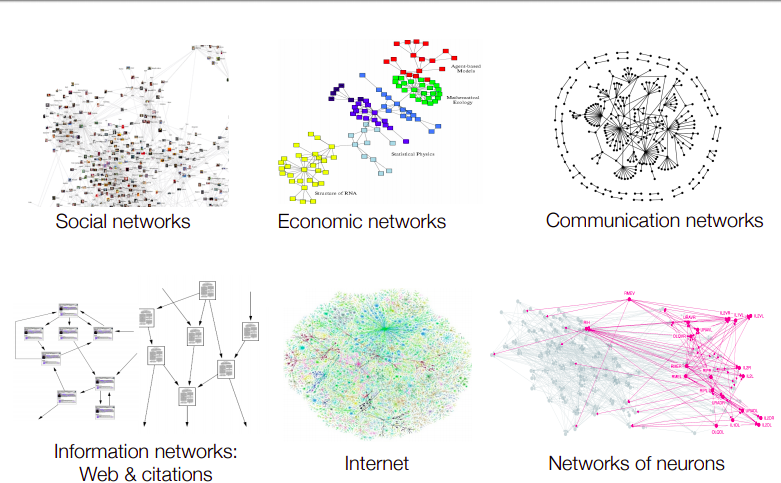
\includegraphics[width=0.7\textwidth]{topics/201010-zhang2019comprehensive/assets/img/real-graph.png}
        \caption{Application}
        \label{fig:application}
    \end{figure}
\end{frame}
\subsection{What is the graph?}
\begin{frame}{What is the graph?}
    \begin{itemize}
        \item G(V, E) ~ Graph, Network, System.
        \item V Vertices ~ Nodes, Objects.
        \item E Edges ~ Link, Interaction.
    \end{itemize}
    \begin{figure}[htp]
        \centering
        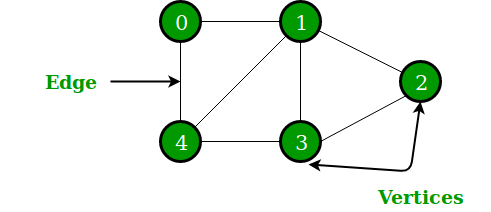
\includegraphics[width=0.7\textwidth]{topics/201010-zhang2019comprehensive/assets/img/graph.png}
        \caption{Graph}
        \label{fig:graph}
    \end{figure}
\end{frame}
\subsection{What is non-Euclidean data?}
\begin{frame}{Graph-based machine learning - What is non-Euclidean data?}
    \begin{block}{What is non-Euclidean data?}
        The shortest path between 2 points isn't necessarily a straight line.
    \end{block}

    \begin{figure}[htp]
        \centering
        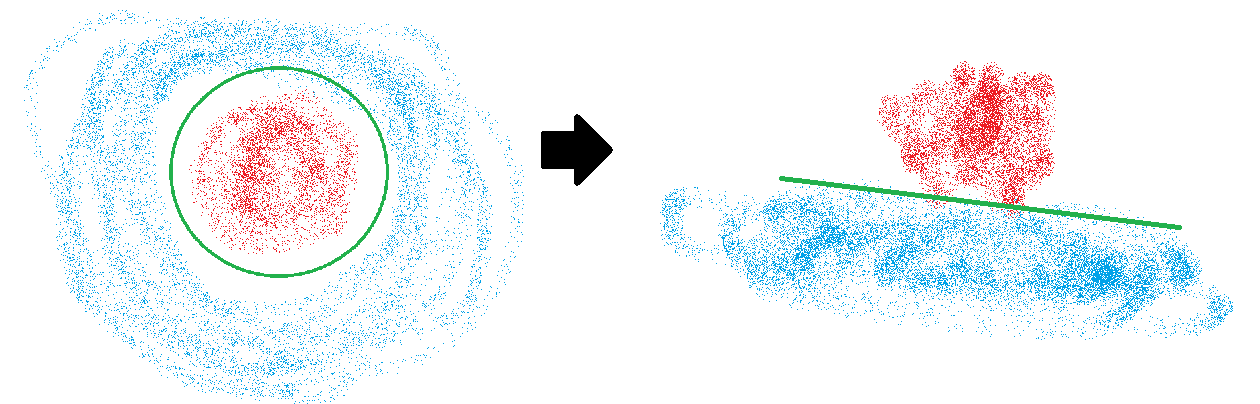
\includegraphics[width=0.8\textwidth]{topics/201010-zhang2019comprehensive/assets/img/concrete_plot.png}
        \caption{Concrete examples}
    \end{figure}
\end{frame}

\subsection{Node2Vec - Embeeding}
\begin{frame}{Graph-based machine learning - Node2Vec - Embeeding}
    \begin{figure}[htp]
        \centering
        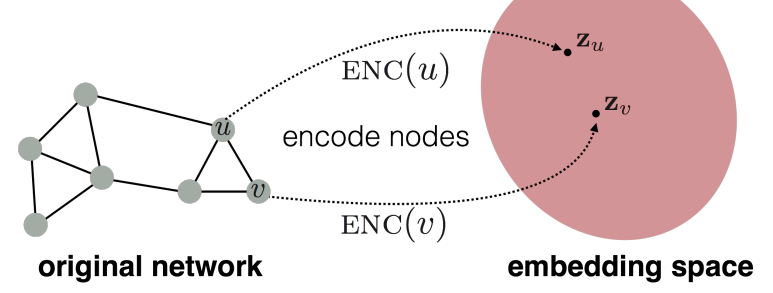
\includegraphics[width=0.8\textwidth]{topics/201010-zhang2019comprehensive/assets/img/euclid_space.png}
        \caption{Embedding}
    \end{figure}
\end{frame}

\begin{frame}{Graph-based machine learning - Node2Vec - Word embeeding}
    \begin{figure}[htp]
        \centering
        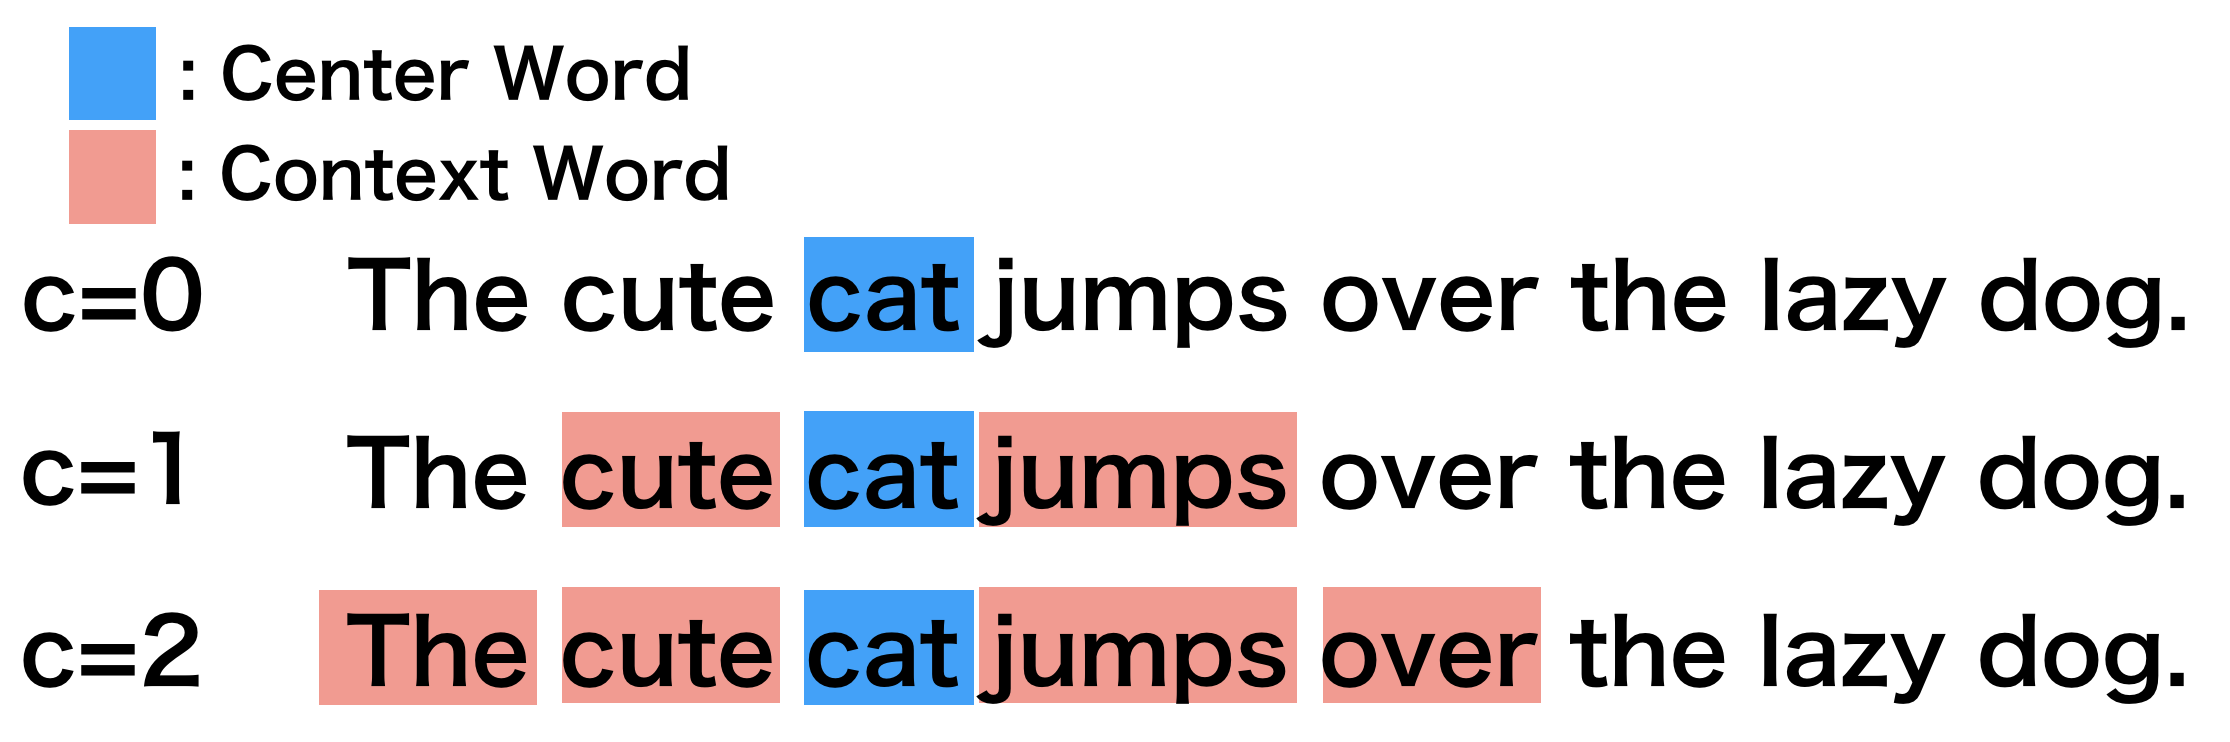
\includegraphics[width=0.8\textwidth]{topics/201010-zhang2019comprehensive/assets/img/context-word.png}
        \caption{Context word}
    \end{figure}
\end{frame}

\begin{frame}{Graph-based machine learning - Node2Vec - Word embeeding}
    \begin{multicols}{2}
        \begin{figure}[htp]
            \centering
            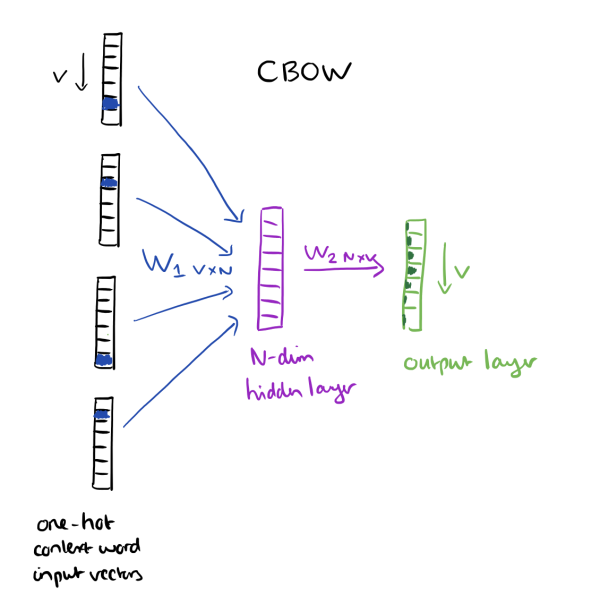
\includegraphics[width=0.4\textwidth]{topics/201010-zhang2019comprehensive/assets/img/cbow.png}
            \caption{CBOW}
        \end{figure}

        \begin{figure}[htp]
            \centering
            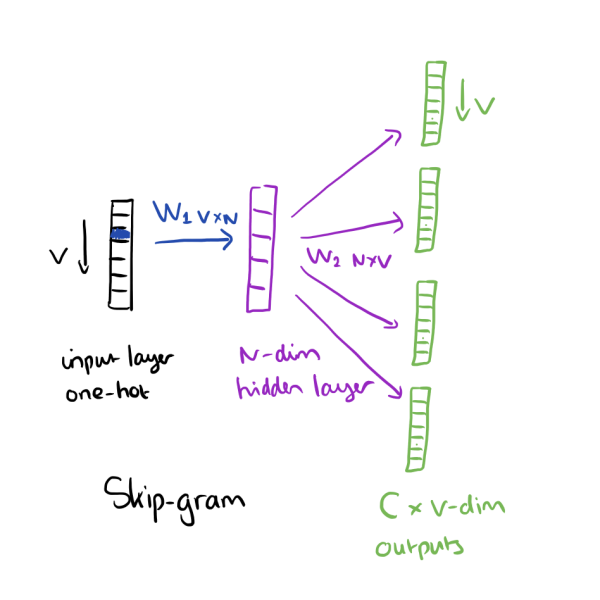
\includegraphics[width=0.4\textwidth]{topics/201010-zhang2019comprehensive/assets/img/skip-gram.png}
            \caption{Skip-gram}
        \end{figure}
    \end{multicols}
\end{frame}

\begin{frame}{Graph-based machine learning - Node2Vec - DeepWalk}
    DeepWalk (Perozzi et al., 2014) is introduced to learn node embeddings via a random walk and word2vec (Mikolo et al., 2013) word2vec algorithm \cite{perozzi2014deepwalk} \cite{mikolov2013distributed}.
    \begin{figure}[htp]
        \centering
        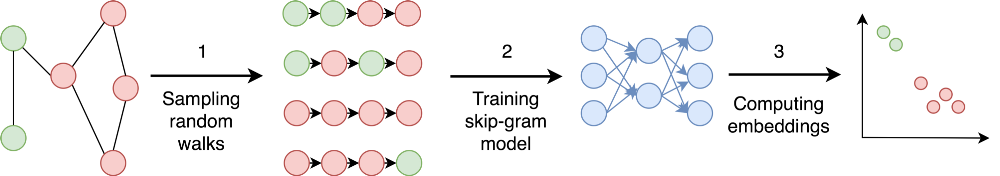
\includegraphics[width=\textwidth]{topics/201010-zhang2019comprehensive/assets/img/deepwalk.png}
        \caption{DeepWalk}
    \end{figure}
\end{frame}

\begin{frame}{Graph-based machine learning - Node2Vec - pq param}
    \begin{figure}[htp]
        \centering
        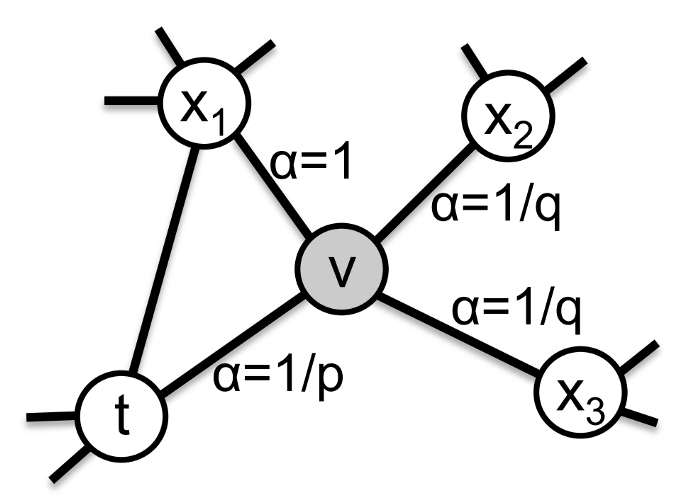
\includegraphics[width=0.6\textwidth]{topics/201010-zhang2019comprehensive/assets/img/p-q-param.png}
        \caption{p q param \cite{grover2016node2vec}}
    \end{figure}
\end{frame}